\section{Background}

\subsection{Petri Nets}

A petri net is a bipartide graph consisting of places, transitions, and arcs where an arc connects a place to a transition or a transition to a place. Generally places are represented by circles and transitions are represented by horizontal lines. In this paper, we will also represent transitions with plaintext giving the action the transition takes. Places from which arcs run to a transition are called input places and places to which arcs run from a transition are called output places. Places in a petri net may contain a discrete number of marks called tokens. A collection of tokens is called a marking. A transition is enabled if there is at least one token at every input place, and that transition may only fire once it is enabled. Upon firing, that transition will consume one token from every input place and generate one token at every output place. A firing is atomic.

A transition that has multiple outgoing arcs is a parallel split, and a transition that has multiple incoming arcs is a parallel merge. A place that has multiple arcs is a conditional split, and a place that has multiple incoming arcs is a conditional merge.

\begin{center}
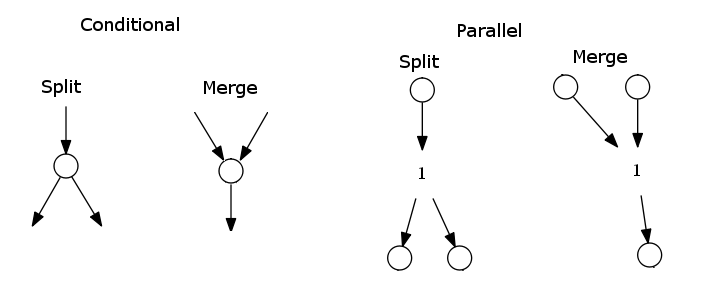
\includegraphics[scale=0.475]{figures/structure.png}
\end{center}

\begin{definition}
A \textbf{state} is a marking such that no token follows another sequentially, no two tokens are on separate banches of the same conditional, and that marking forms a complete graph cut across all parallel branches.
\end{definition}

\begin{definition}
A \textbf{partial state} is a marking such that no token follows another sequentially and no two tokens are on separate banches of the same conditional.
\end{definition}

\begin{center}
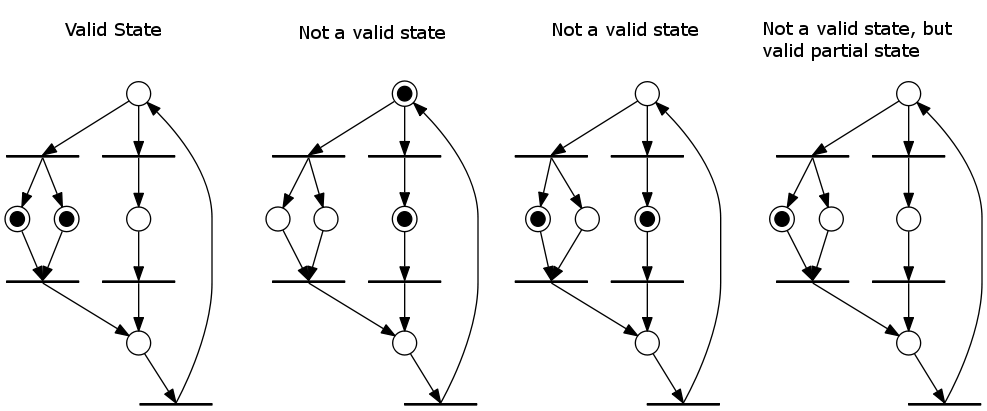
\includegraphics[scale=0.475]{figures/state.png}
\end{center}

\subsection{Hand Shaking Expansions}

Hand shaking expansions are represented by petri nets modified in the following way.

\begin{definition}
A \textbf{state encoding} is a value assignment of either true or false for every node in the circuit represented by the hand shaking expansion.
\end{definition}

\begin{definition}
A \textbf{predicate} is a boolean expression which represents the set of possible state encodings for a given marking. A marking and its predicate will be represented by the same symbol.
\end{definition}

\begin{definition}
A \textbf{transition expression} is a boolean expression representing the action that a transition takes. A transition and its expression will be represented by the same symbol.
\end{definition}

Boolean operators and set operators are interchangable when dealing with predicates and transition expressions. Given two boolean expressions $E_0$ and $E_1$ and the two sets of state encodings they represent $S_0$ and $S_1$:
\begin{itemize}
\item $S_0 \cap S_1 \equiv E_0 \wedge E_1$
\item $S_0 \cup S_1 \equiv E_0 \vee E_1$
\item $S_0^C \equiv \neg E_0$
\item $S_0 \subset S_1 \equiv E_0 \wedge E_1 = E_0$
\end{itemize}
For the purpose of this paper in all cases, I will use the boolean operators except when I want the subset in which case I will use the set operator.

\begin{definition}
\textbf{Active transitions} represent assignments. The transition expression for an active transition represents a value assignment for a single node. When an active transition fires, it changes the value assignment for that node in all state encodings represented by a given boolean expression. The action taken by an active transition will represented by the `$\rightarrow$' operator.
\end{definition}

\begin{lemma}
$(A \vee B) \rightarrow T = (A \rightarrow T) \vee (B \rightarrow T)$
\end{lemma}

\begin{lemma}
$(A \wedge B) \rightarrow T = (A \rightarrow T) \wedge (B \rightarrow T)$
\end{lemma}

\begin{lemma}
$\neg (A \rightarrow T) = \neg A \rightarrow \neg T$
\end{lemma}

\begin{definition}
\textbf{Passive transitions} represent guards. The transition expression for a guard may be any boolean expression. For a passive transition $T$ to fire given the current state $S_i$, $S_i \wedge T \ne false$ meaning there is at least one state encoding represented by the predicate of $S_i$ that satisfies the condition given by $T$. This also means that a passive transition may be enabled, but is unable to fire. When a passive transition fires, the predicate for the new state, $S_{i+1} = S_i \wedge T$. If $T$ has multiple minterms $T_j$ such that $S_i \wedge T_j \ne false$, then each of those terms must be considered in independent executions.
\end{definition}

\begin{definition}
A transition $T$ with input places $P_{in}$ and output places $P_{out}$ is \textbf{definitely vacuous} if
\begin{align}
 \bigwedge_{P_o \in P_{out}} P_o = \bigwedge_{P_i \in P_{in}} P_i
\end{align}
\end{definition}

\begin{definition}
A transition $T$ with input places $P_{in}$ and output places $P_{out}$ is \textbf{possibly vacuous} if
\begin{align}
 \bigwedge_{P_o \in P_{out}} P_o \wedge \bigwedge_{P_i \in P_{in}} P_i \ne false
\end{align}
\end{definition}

\begin{lemma}
All passive transitions are either possibly or definitely vacuous.

By definition of passive transition, the predicate of the output places of a passive transition is always a subset of the predicate of the input places.
\end{lemma}

\begin{lemma}
All of the output transitions of a conditional split will be passive.

The only case in which a conditional would not have a guard is when the guard is $true$. However if the guard is $true$, then there can only be one guard and therefore it is not a conditional split.
\end{lemma}

There are also some restrictions that must be maintained in order for this to work. First, a transition with multiple incoming arcs or multiple outgoing arcs must be definitely vacuous (preferably $T \equiv true$). Second, a transition cannot have both multiple incoming arcs and multiple outgoing arcs. This means that you cannot have a parallel merge in the same transition that you also have a parallel split. These two requirements guarantee that all conflicting state pairs are detectable and that it is possible to insert a state variable transition between any two transitions, splits, or merges by cutting exactly one arc. Finally, proper nesting is required for conditional splits and merges, but not required for parallel splits and merges, and the initial marking must be a state that is not on a conditional branch. This requirement allows for correct simulation of the hand shaking expansion.



